\section{Architecture}

\begin{figure}[t]
   \begin{center}
     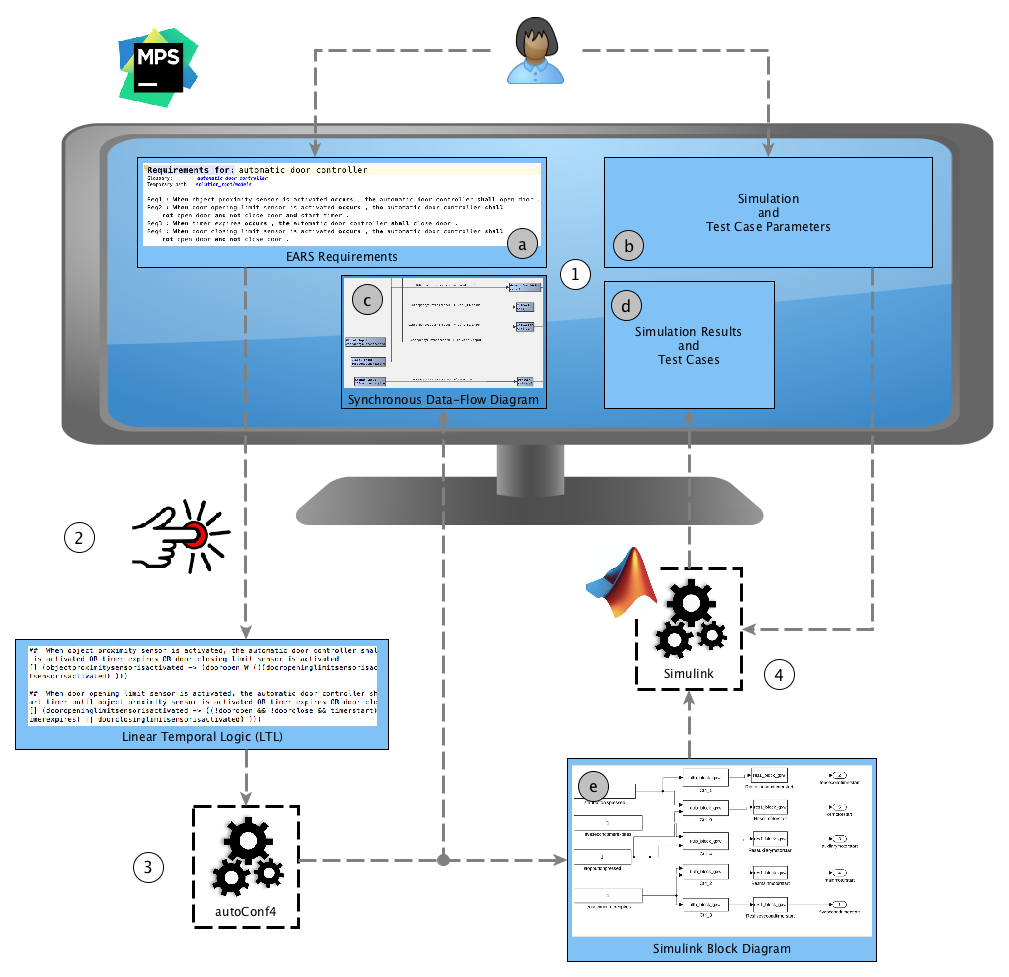
\includegraphics[width=1\textwidth]{images/toolchain.png}
     \caption{The \textsf{EARS-CTRL} Tool Chain}
     \label{fig:ears_ctrl_toolchain}
   \end{center}
 \end{figure}
 
In figure~\ref{fig:ears_ctrl_toolchain} we depict the architecture of the
\textsf{EARS-CTRL} tool. In the following paragraphs we will provide to the
reader a brief description of the main components of the tool's architecture,
how those components have been implemented and which artifacts those
components interchange. 
 
\paragraph{1. EARS and Glossary Editor\\\\} 

As previously mentioned, an \textsf{EARS-CTRL} specification is composed of a
Glossary and of a set of requirements.

Additionally, in the glossary the requirements engineer can also express
relationships between signals such that necessary constrains can be defined, as show in figure~\ref{}.

Aliases for signals can also be defined, as can be seen in figure~\ref{}. These
aliases are helpful in making the specification readable, as can be seen in the
example in figure~\ref{}.

\paragraph{2. From EARS to Lineal Temporal Logic\\\\}

\paragraph{3. Synthesizing a Controller using \textsf{autoConf4}\\\\}

In order to achieve such as synthesis we
use the \textsf{autoConf4} tool, which takes as input as set of LTL and
propositional logic formulas. In figure~\ref{} we depict the translation of the
automatic door specification in figure~\ref{} into LTL. Note that the
translation is not directly one-to-one from EARS requirements into LTL formulas,
as some details are added by the translation algorithm in order to take into
consideration particularities of the \textsf{autoConf4} tool. This can be
observed \ldots.

\paragraph{4. Simulation and Test Case Generation Control Panel\\\\}

 In figure~\ref{} we display the panel that allows ``playing'' the
controller by providing a sequence of inputs manually. Outputs are incrementally
added to the panel as new inputs are provided by the requirements engineer.
Note that the controller keeps state, which means that the order in which the commands are given matters.
The ``Reset'' button in the panel allows resetting the controller to its initial
state.

Say here how the exploration mechanism works by simulating steps iteratively to
build the test cases according to the test set parameterization.

\paragraph{5. Simulation and Test Generation using Simulink\\\\}

Talk about how blocks from simulink are composed together to allow building the
expected behavior. Some blocks had to be purposefully build to allow simulation
to happran. This is done via a script that loads the model into simulink \ldots
